\documentclass[11pt,ngerman]{scrartcl}

% standard packages
\usepackage[utf8]{inputenc}  % input in UTF-8
\usepackage[T1]{fontenc}  % output in T1 fonts (westeuropäische Codierung)
\usepackage{lmodern}  % latin modern fonts
\usepackage[ngerman]{babel}  % deutsches Sprachpaket, neue Rechtschreibung

% Seitensetup
\usepackage{scrlayer-scrpage}  % Seitenformatierung durch KOMA-interne Optionen
\usepackage[top=4cm, bottom=4cm]{geometry}  % Seitengeometrie (kann durch KOMA ersetzt werden, hab ich aber nicht geschafft)
\usepackage[hypcap=false]{caption, subcaption}  % caption editing - hypcap warning with hyperref
\usepackage{array}  % table editing

% additional packages
\usepackage{amsmath, amssymb, amstext}  % math packages (American Math Society)
\usepackage{bm}
\usepackage{icomma}  % Kommata in Dezimalzahlen verursachen keinen Abstand mehr
\usepackage{graphicx}  % Bilder einfügen
\usepackage{float} %Bilder placement
\usepackage{pdfpages}  % PDF als vollständige Seiten einfügen
\usepackage{lastpage}  % referenziert die letzte Seite
\usepackage[separate-uncertainty=true]{siunitx}  % bessere Darstellung von Einheiten
\usepackage{makecell} %Dicke Tabellenstriche
\usepackage{longtable}
\usepackage{booktabs}
%\usepackage{datatool}
\usepackage[hidelinks]{hyperref}  % hyperref verlinkt Referenzen - hidelinks entfernt borders um links

% package setups
% Kopf- und Fußzeile durch KOMA
\pagestyle{scrheadings}  % KOMA darf entscheiden
\clearpairofpagestyles  % reset
\setkomafont{pageheadfoot}{\normalfont}  % Standardschrift in Kopf- und Fußzeile
\captionsetup{format=plain, font=small, labelfont=bf} %Better caption, Abbildung ist FETT
%\setlength{\headheight}{27.2pt}  % benötigte Höhe Kopfzeile (warning von scrlayer-scrpage, wird aber automatisch so gerendert, falls diese Option weggelassen wird)
\ihead{Reibung}  % Kopf links %Todo Titel ändern
\chead{\textsc{Philipp} Maximilian}  % Kopf Mitte %Todo Name ändern
\ohead{06 Juli 2021}  % Kopf rechts %Todo Datum ändern
\cfoot{\pagemark \, / \pageref{LastPage}}  % Fuß Mitte

% Table of Contents
\DeclareTOCStyleEntry{dottedtocline}{section}  % KOMA intern - Inhaltsverzeichnis mit Punkten (nur sections)

%Overbar setup
\newcommand{\overbar}[1]{\mkern 1.5mu\overline{\mkern-1.5mu#1\mkern-1.5mu}\mkern 1.5mu}
% SI
\sisetup{locale = DE}  % deutschsprachige SI-Konvention
\sisetup{quotient-mode = fraction}
\sisetup{per-mode = fraction}
\DeclareSIUnit\px{px}

% citation
\usepackage{csquotes}
\usepackage[backend=biber]{biblatex}
\addbibresource{pics/reibung.bib} %Todo .bib befüllen zb.: mit JabRef (Empfehlung der Redaktion)

% array
\renewcommand{\arraystretch}{1.2}

\begin{document}

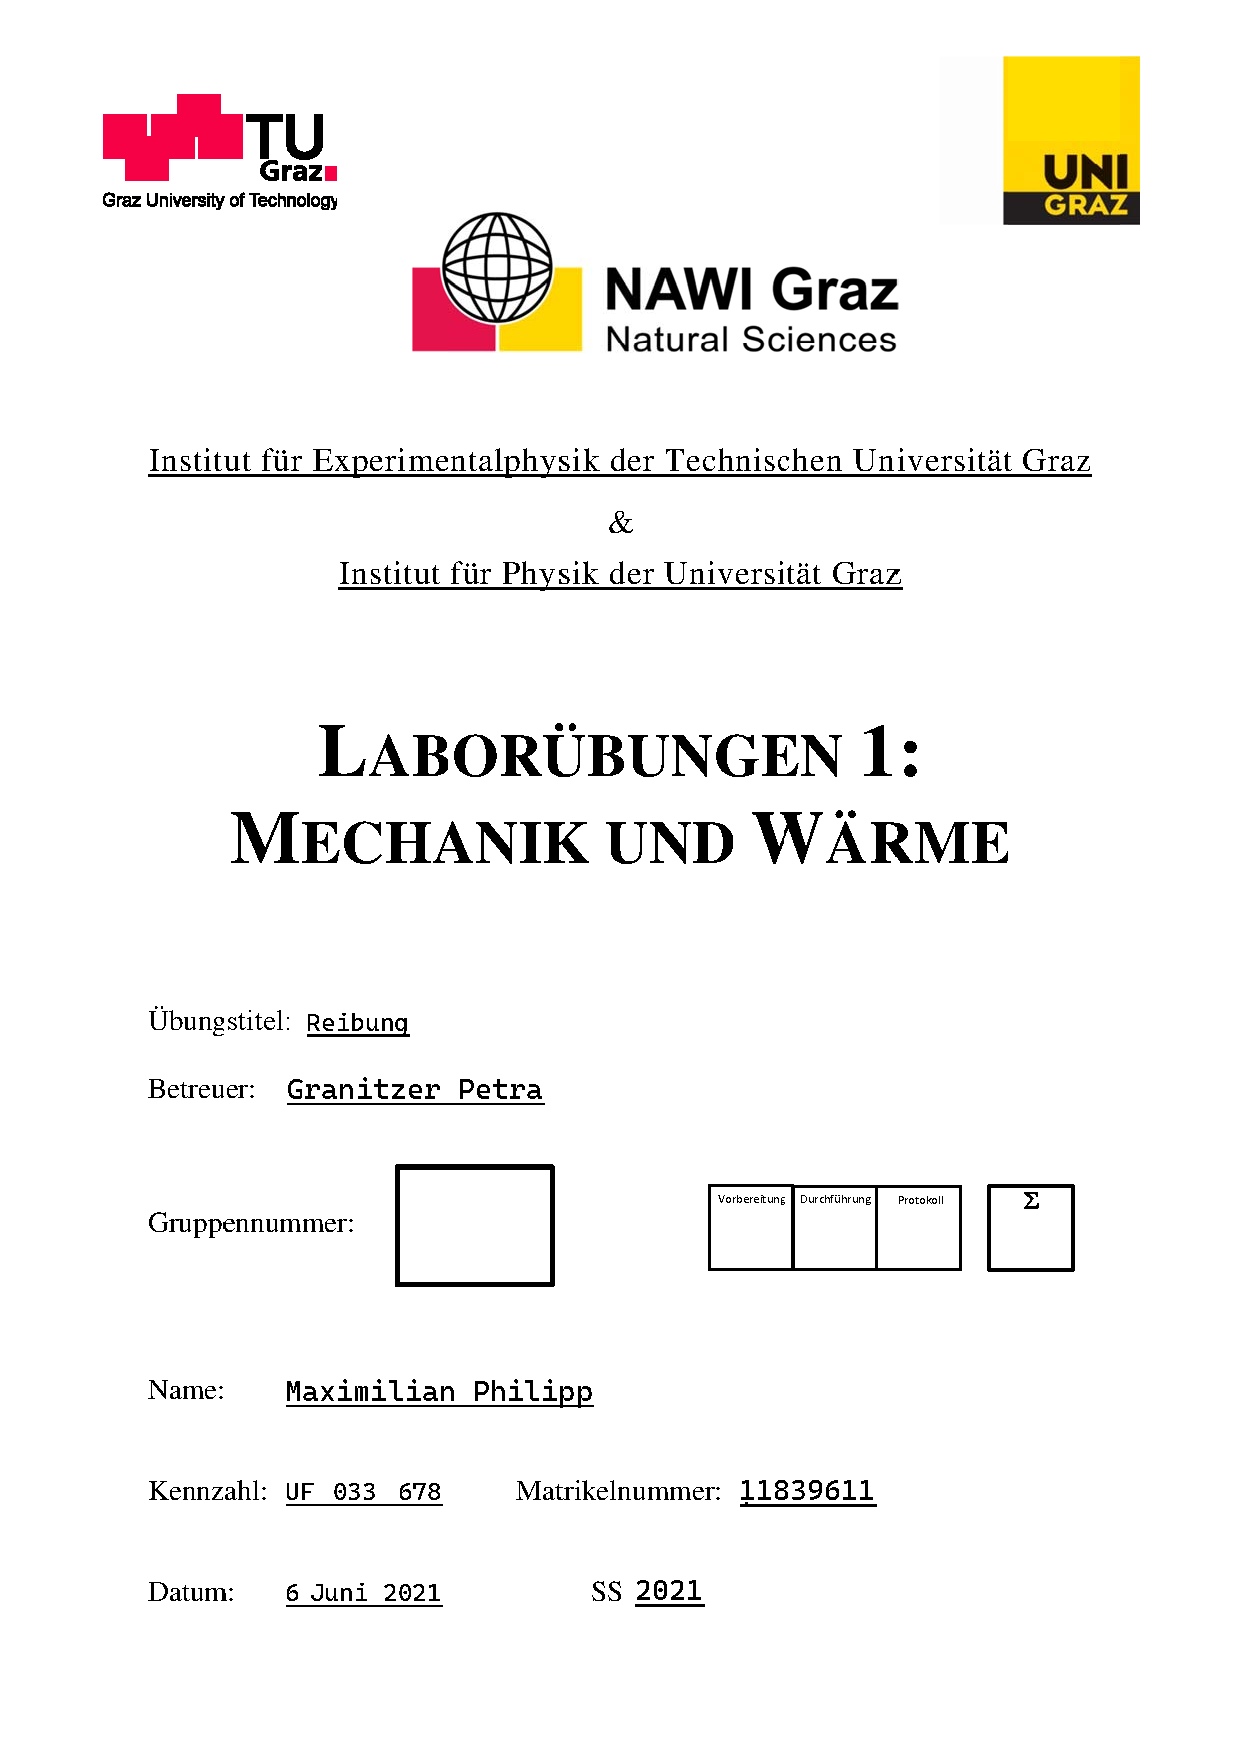
\includepdf{pdfs/Deckblatt.pdf} % Todo Deckblatt ausfüllen
%\title{Reibung}
%\author{\textsc{Philipp} Maximilian\\11839611}
%\date{06.06.2021}
%\maketitle

\tableofcontents
\newpage
\section{Aufgabenstellung}
\label{sec:aufgabenstellung} 

\begin{enumerate}
    \item  Bestimmung der Koeffizienten der Haft-, Gleit- und Rollreibung
        und deren Einfluss auf die Bewegung von Körpern.
    \item Bestimmung der Viskosität einer zähen Flüssigkeit.
    \item Auswertung am Computer (python).
\end{enumerate}

\section{Voraussetzungen und Grundlagen} \label{sec:voraussetzungen_grundlagen}
Folgende Grundlagen wurden aus dem Mechanik Vorlesungsskript \cite{Knoll2020}
entnommen und für dieses Experiment leicht angpasst.

\subsection{Reibung}

Für folgende Gleichungen bei einer schiefen Ebene ist
$l$ der Teil der Länge des Brettes, welcher noch nicht über die Buchkanten
herausragt, und die Buchstapelhöhe $h$. Diese zwei Seiten bilden
ein rechtwinkliges Dreieck, welches $l$ als Hypothenuse und $h$
als Gegenkathete hat. Mit Hilfe des Satzes von Pythagoras lässt
sich ein Ausdruck für den Tangens vom Winkel $\alpha$ zwischen der Hypothenuse
und der Ankathete finden:

\begin{equation}
    \tan{\alpha} = \frac{h}{\sqrt{l^2-h^2}} \label{eq:tangens}
\end{equation}

\begin{figure}[H]
    \centering
    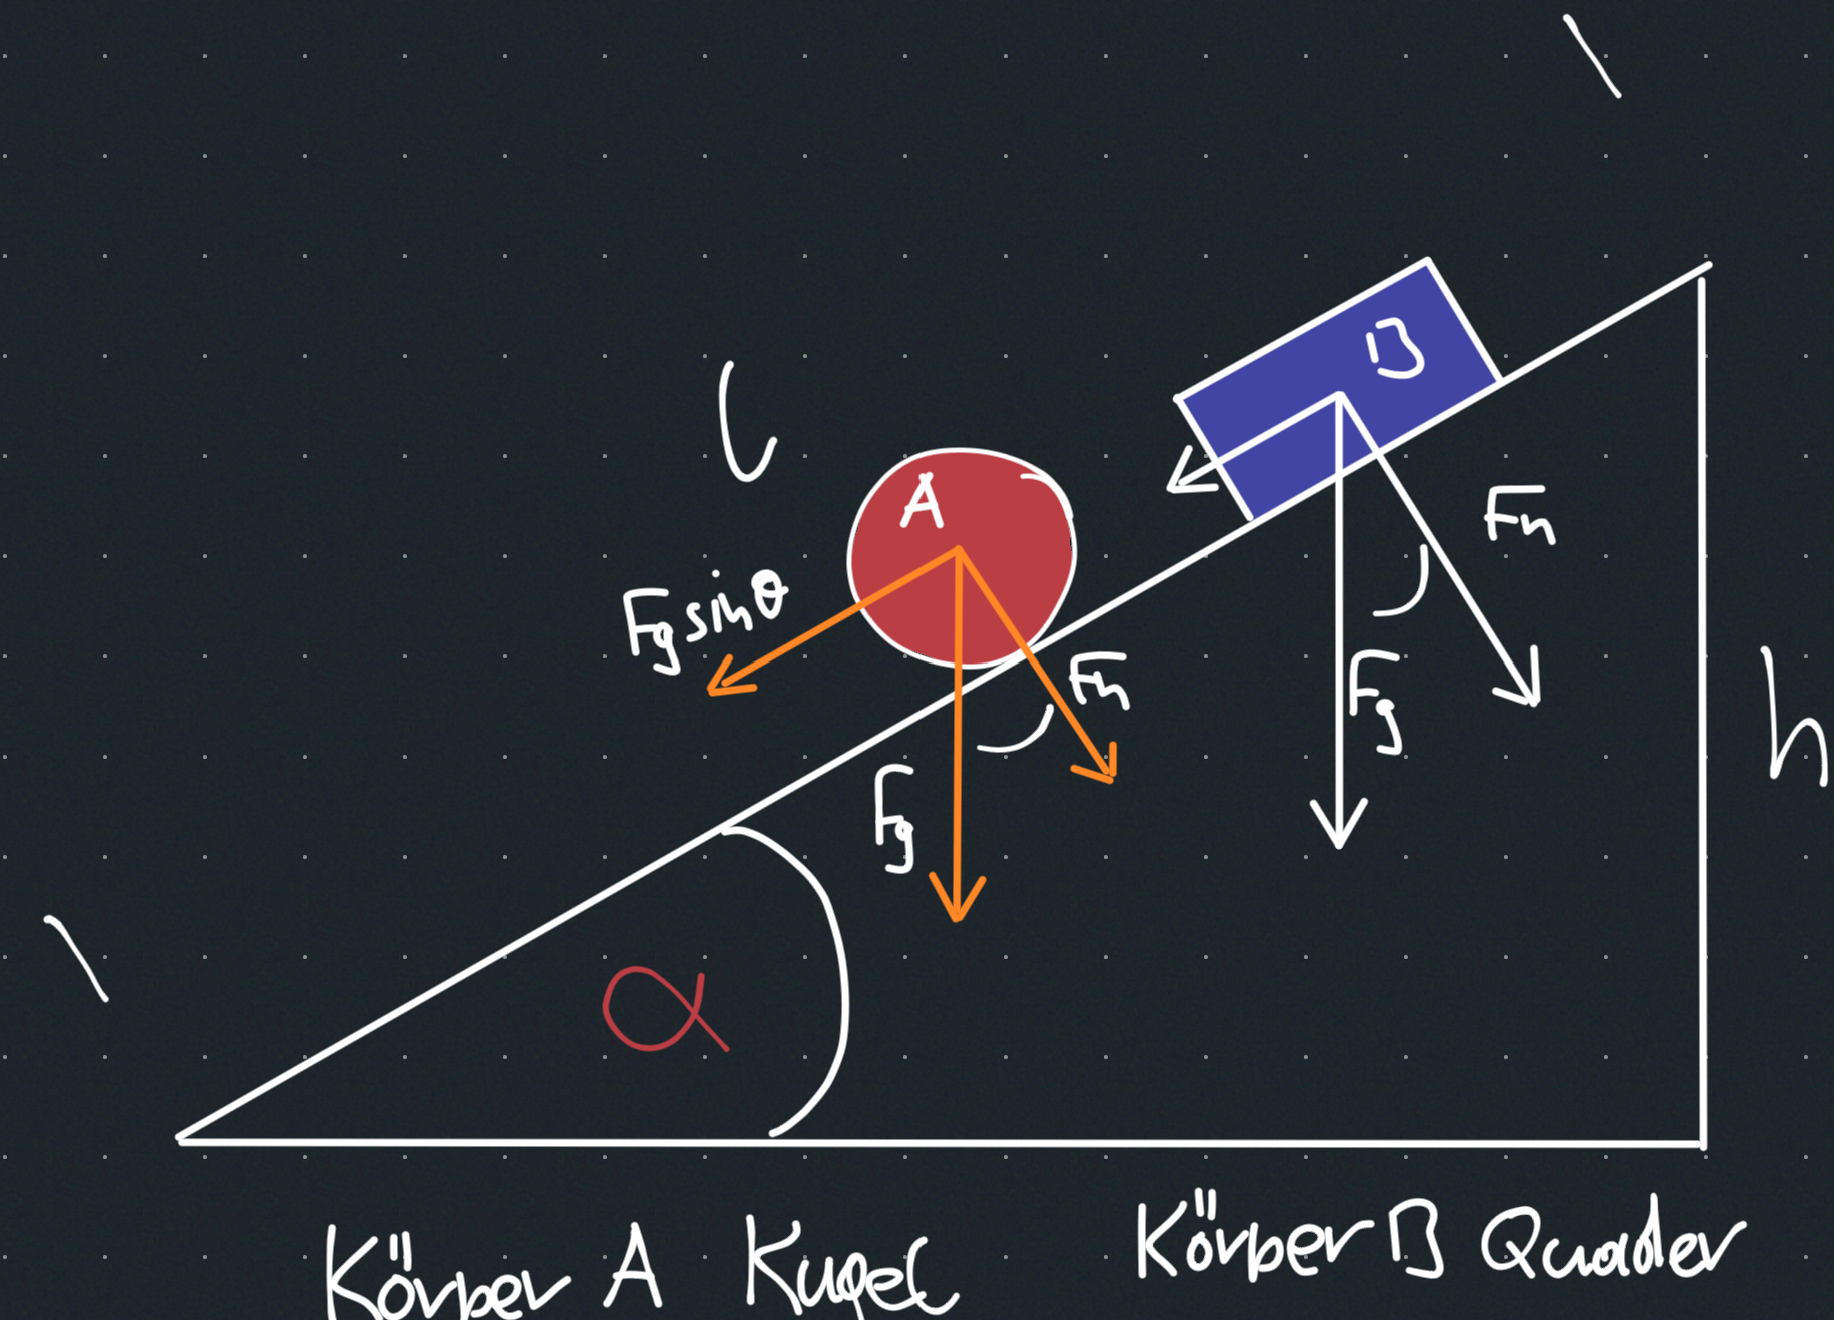
\includegraphics[width=0.8\linewidth]{pics/Skizze.png}
    \caption{Diese Skizze soll die Bedeutung der Variablen im Kontext des Experiments 
    visuell darstellen}%
    \label{fig:Skizze}
\end{figure}

Ziel dieses Experiments ist die Bestimmung der Haft-, Gleit- und
Rollreibungskoeffizienten von zwei Festkörpern, in diesem Fall von einem
Gummiball und einer Handyhülle aus PET. Weiters ist noch die Viskosität einer
Flüssigkeit zu bestimmen. In diesem Protokoll werden die üblichen Abkürzungen
für diese Koeffizienten verwendet: $\mu_H$ für den Haft-, $\mu_G$ für den Gleit- und $\mu_R$
für den Rollreibungskoeffizienten \cite{Knoll2020}.

Die Normalkraft $F_N$ bei der schiefen Ebene ist:
\begin{equation}
    F_N = mg \cos(\alpha) \label{eq:FN_schiefebene}
\end{equation}

Wobei $m$ die Masse des Objekts und $g$ die Erdbeschleunigung ist, diese
Kraft sieht man gut in \autoref{fig:Skizze}.

Nun lässt sich die Haftreibung $R_H$ proportional zur Normalkraft definieren,
wobei die Proportionalitätskonstante der Haftreibungskoeffizient $\mu_H$ ist.

\begin{equation}
    R_H = \mu_H F_N \label{eq:haftreibungkraft}
\end{equation}

Setzt man nun ein Objekt auf eine flache Ebene und beginnt sie zu heben, hindert
die Haftreibung das Objekt daran sich zu bewegen. Wird jedoch die treibende
Kraft $F_t = mg \sin(\alpha)$ größer als die Haftreibung, setzt sich das Objekt
in Bewegung. Es existiert ein Winkel bei dem die Kräfte sich kompensieren, also
ein Kräftegleichgewicht:
\begin{equation}
    R_H = mg \sin(\alpha)
\end{equation}

Findet man durch Messen den gesuchten Winkel $\alpha$, kann daraus der
Haftreibungskoeffizient $\mu_H$ bestimmt werden.

\begin{equation}
    \mu_H = \tan(\alpha) = \frac{h}{\sqrt{l^2-h^2}} \label{eq:haft}
\end{equation}

Befindet sich das Objekt schon in Bewegung, liegt eine andere Art der Reibung vor,
die Gleitreibung $R_G$, welche sich auch proportional zur $F_N$ schreiben lässt.

\begin{equation}
R_G = \mu_G F_N \label{eq:gleit_ansatz}
\end{equation}

Da sich hier die Kräfte nicht kompensieren, existiert eine Restkraft $F$, welche 
das Objekt dazu veranlässt sich zu beschleunigen.

\begin{equation}
    F = m\ddot{x} = mg \sin(\alpha) - R_G = mg \sin(\alpha) - \mu_G mg \cos(\alpha) \label{eq:krafgleit}
\end{equation}

Unter Annahme einer gleichmäßigen Beschleunigung und $v_0=0$ lässt sich für die
Beschleunigung $\ddot{x}$ folgender Ausdruck $\ddot{x} = \frac{2s}{t^2}$
einsetzen. Formt man nun \autoref{eq:krafgleit} auf $\mu_G$ um, erhält man folgende Formel:

\begin{equation}
    \mu_G = \tan(\alpha)-\frac{2s}{gt^2 \cos{\alpha}} = \mu_H - \frac{2s}{gt^2 \cos{\alpha}} \label{eq:gleit}
\end{equation}

Die Rollreibung $\mu_R$ ist, wie im Vorlesungskript der Mechanik und
Wärme \cite{Knoll2020}, über das Drehmoment definiert.
Das Drehmoment ist das Drehmoment, welches vonnöten ist eine Kugel (oder Zylinder) in Bewegung
zu setzen. Der Rollreibungskoeffiziente $\mu_R$ ist
die Proportionalitätskonstante zwischen der Normalkraft $F_N$
und dem zuvor erwähnten Drehmoment $D_R$, somit
hat der Rollreibungskoeffiziente die Einheit einer
Länge. Das Drehmoment ist der Radius $r$ der Kugel kreuz der
Treibenden Kraft $F_R$, da diese Kräfte orthogonal auf einander
stehen, ist einfach multipliziert worden.
Da $F_N$ und $F_R$ die Komponenten
der Gravitationskraft sind, existiert eine Winkelabhängigkeit.
Diesen Winkel gilt es nun zu bestimmen.

\begin{equation}
    D_R = F_R r = rmg \sin(\alpha) = \mu_R F_N = mg \cos(\alpha)
\end{equation}

Formt man auf $\mu_R$ um, erhält man folgende \autoref{eq:roll}:

\begin{equation}
    \mu_R = r \tan(\alpha) = r \frac{h}{\sqrt{l^2-h^2}}  \label{eq:roll}
\end{equation}


%$E_{reib} = D_R \phi = \mu_R F_N \frac{s}{r}$
%
%$E_{roll} = \frac{I \omega^2}{2}$
%
%$I = \frac{2}{5} m r^2 + m r^2 = \frac{7}{5} m r^2$
%Kein Schlupf
%
%$\text{d}s = r \text{d}\phi$
%
%$E_{pot} = mgh$
%Energieerhaltung
%
%$E_{pot} = E_{roll} + E_{reib}$
%
%All die ins System gesteckte System gesteckte muss 
%in eine gewisse Art und Weise in Reibung umgewandelt.
%Hier wird die Annahme gemacht, dass die Rollreibung
%die einzige Reibung ist die hier Effekt trägt. Also
%keine Reibung die von der Geschwindigkeit abhängt.
%Diese Annahme lässt sich machen wenn Objekt sich
%langsam bewegen. Daraus folgert, dass die, durch die
%Reibung ``verlorengegangene'', Energie nur 
%von dem zurückgelegten Weg abhängt.
%
%Dadurch lässt sich ein Ausdruck für die Rollreibung $\mu_R$ finden:
%
%\begin{equation}
%    \mu_R = \frac{I\omega^2 r}{2 F_N s} 
%\end{equation}
%
%Schwingungsgleichung:
%
%$m\ddot{x} + \omega^2 x = - F_R$

\subsection{Viskosität}

Nun zur Theorie für die Viskosität:

Wenn sich eine Kugel durch eine zähe Flüssigkeit durchbewegt, spürt diese 
eine Kraft, welche proportional zu der Bewegungsgeschwindigkeit $v$ ist.
Diese Reibungkraft entspricht dem Stokes'schen Gesetz, welche \autoref{eq:stokes}
der Viskosität $\eta$ der Flüssigkeit, dem Radius der Kugel $r$ und 
wie zuvor erwähnt von der Bewegungsgeschwindigkeit $v$ abhängt.

\begin{equation}
    F_R = -6\pi\eta r v \label{eq:stokes}
\end{equation}

Bewegt sich eine Kugel durch ein Medium, wirkt nicht nur die Stokes'sche Reibung,
sondern auch der Auftrieb, welcher durch die verdrängte Masse verursacht wird.
Es stellt sich also ein Kräftegleichgewicht ein, wo die Auftriebskraft
$F_A=\rho_{Medium}Vg$ ($V$ das Volumen der Kugel, $g$ die Erbeschleunigung und
$\rho_{Medium}$ die Dichte des Mediums ist) mit der Stokes'schen Reibung $F_R$
der Gravitationskraft $F_G=mg$ ($m$ Masse der Kugel und $g$ die
Erbeschleunigung) entgegen wirken.
$F_A + F_R = F_G$

Setzt man nun in die Gleichung ein und formt auf die Viskosität $\eta$ um, 
erhält man folgende \autoref{eq:viskositat}:

\begin{equation}
    \eta = \frac{2r^2 g (\rho_{Kugel}-\rho_{Medium})}{9v} \label{eq:viskositat}
\end{equation}

Wobei $r$ der Radius der Kugel, $\rho_{Kugel}$ die Dichte der Kugel, $g$ die
Erdbeschleunigung und $\rho_{Medium}$ die Dichte des Mediums ist.

Aus der Zähigkeit lässt sich noch die Reynold Zahl Re des Experiments bestimmen:

\begin{equation}
    \text{Re} = \frac{\rho vd}{\eta} 
\end{equation}

Wo $\rho$ die Dichte des Mediums, $d$ der Durchmesser der Kugel und
$v$ die Fallgeschwindigkeit ist.

Um zu sehen wie sich die Unsicherheit der Messungen bis in die Ergebnisse 
fortpflanzt, ist \autoref{eq:Unsicherheitsfortpflanzung} verwendet worden.
Die Grundlagen dieser Gleichung sind von den Powerpointfolien von 
GUM entnommen worden.\cite{WolfgangKessel2004} Die Verallgemeinerung stammt von Wikipedia \cite{2020Fehler}.
Für die Auswertung ist die Progammiersprache Python im speziellen das 
Packet \verb#scipy#, zur Hilfe genommen worden.

\begin{equation}
    \label{eq:Unsicherheitsfortpflanzung}
    V_y = J(x) \cdot V_x \cdot J^{T}(x)
\end{equation}

Wobei $V_y$ und $V_x$ die Kovarianzmatrizen von den Vektoren $\bm{y}$ und $\bm{x}$.
$\bm{x}$ ist der Vektor der Eingangsvariablen und $\bm{y}$ ist der Vektor der Ausgangsvariablen.
$J$ ist die Jakobimatrix der vektorwertigen Funktion $\bm{y} = \vec{F}(\bm{x})$.
So lassen sich die Komponenten der Matrix relativ einfach anschreiben $J_{ij}(x) = \frac{\partial{y_i}}{\partial{x_j}}(x)$.
Damit man die Unsicherheit der einzelnen Variablen $y_i$ bekommt, muss nur die Quadratwurzel des i-ten Diagonalelementes der 
$\bm{y}$-Kovarianzmatrix genommen werden $u_i= \sqrt{\mathrm{diag}(V_y)_i}$.
Da in diesem Experiment meistens nur skalare Funktionen untersucht werden, vereinfacht
sich die \autoref{eq:Unsicherheitsfortpflanzung} dramatisch und die Unsicherheit
der Variable $y$ lässt sich einfach so berechnen:

\begin{equation}
    \label{eq:graduncentainty}
    u_y = \sqrt{\mathrm{grad} y^T \cdot V_x \cdot \mathrm{grad} y}
\end{equation}

\section{Versuchsanordnung}
\label{sec:versuchsanordnung}

Ein Brett wird so auf einen Stapel von Bücher gelegt, dass die Kante des
Brettes auf den festen Buchrücken liegt, siehe \autoref{fig:buchstapel},
damit die Länge der Hypothenuse dieses rechtwinkligen Dreiecks genau bekannt ist.
Dieser Aufbau wird verwendet um verschiedene Reibungskoeffizienten von Gummi
zu bestimmen.

\begin{figure}[H]
    \centering
    \begin{minipage}[htbp]{\linewidth}
        \begin{minipage}[htbp]{.65\linewidth} % [b] => Ausrichtung an \caption
            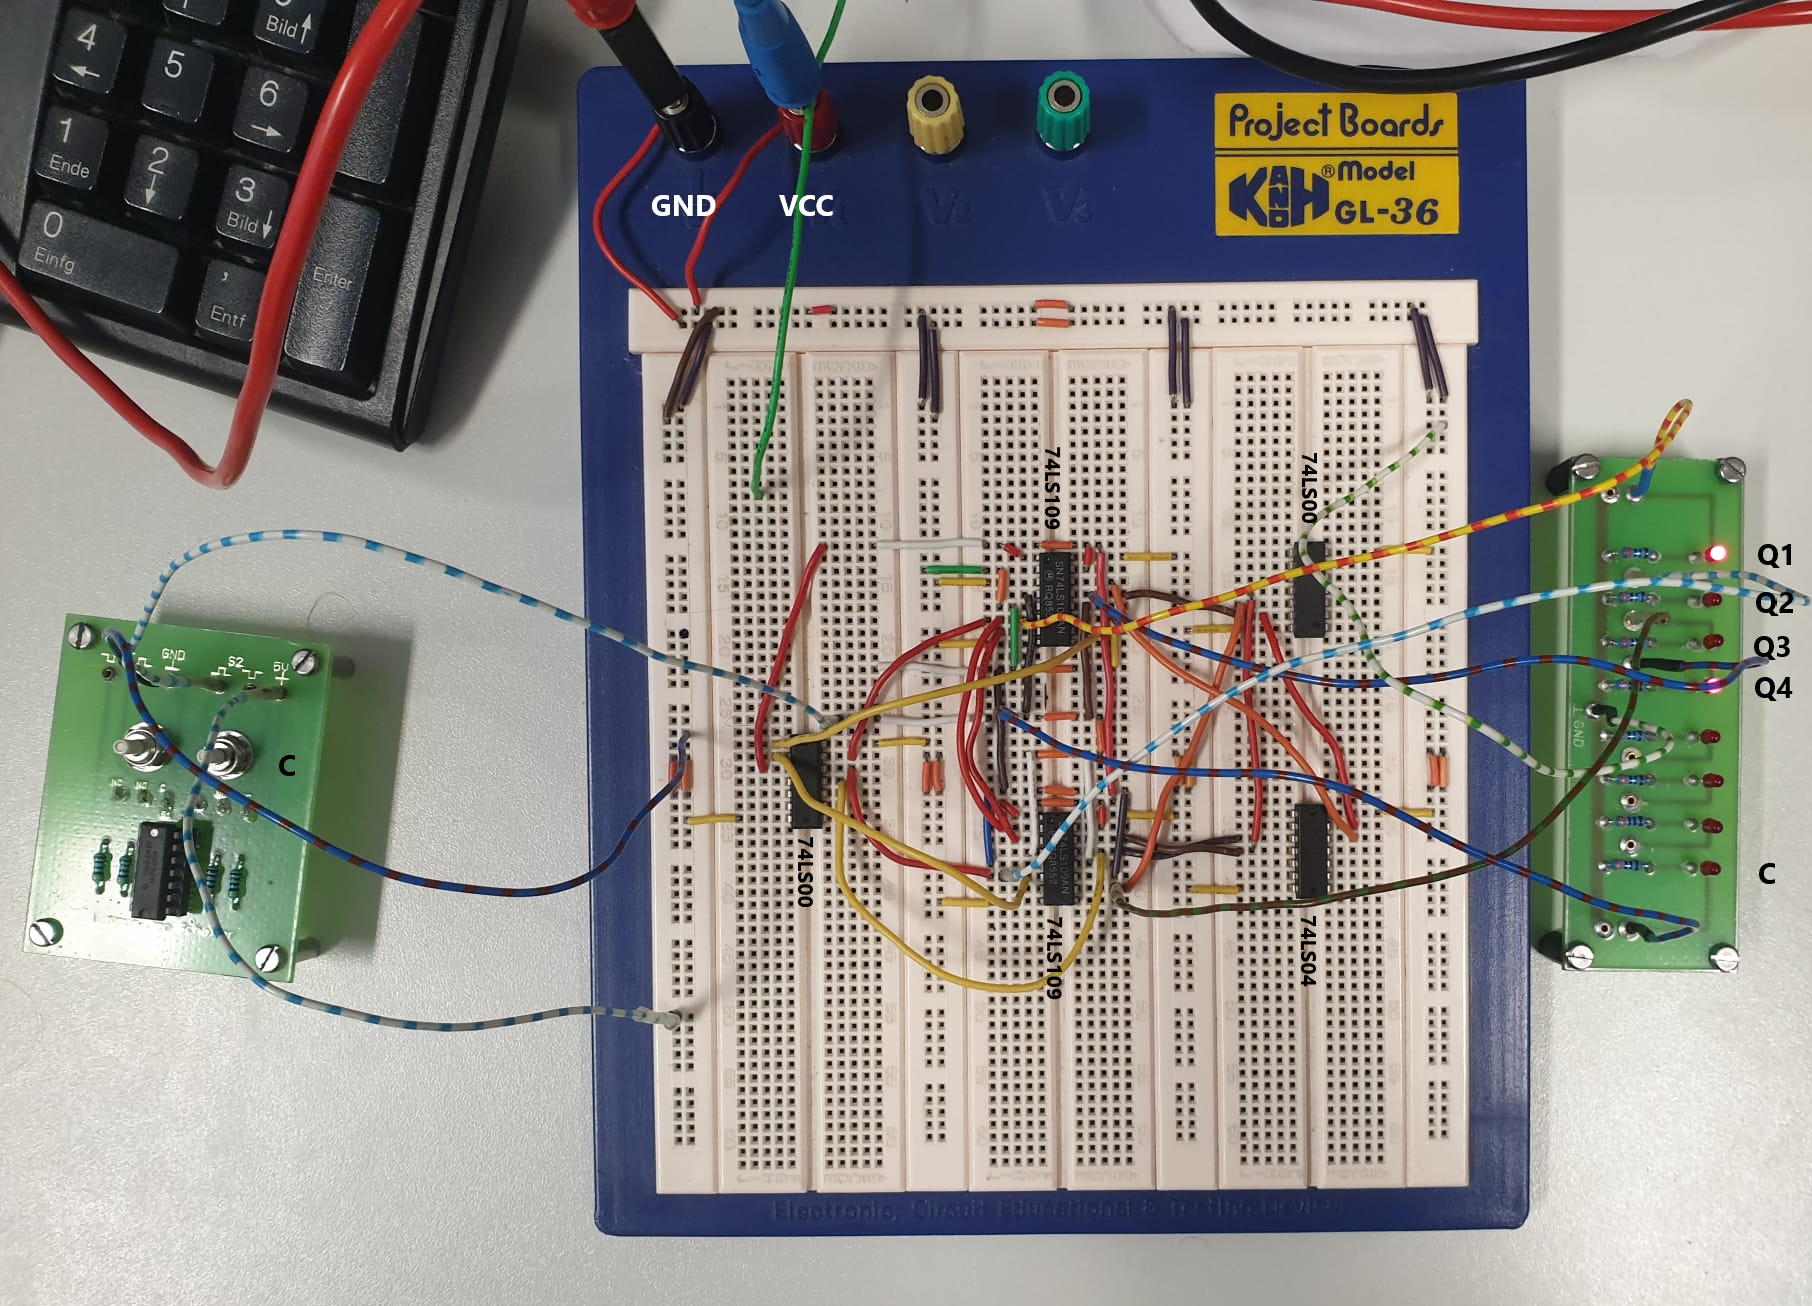
\includegraphics[width=\linewidth]{pics/aufbau.png}
        \caption[Aufbau des Experiments]{Aufbau des Experiments der schiefen Ebene.}
        \label{fig:aufbau}
        \end{minipage}
        \begin{minipage}[htbp]{.30\linewidth} % [b] => Ausrichtung an \caption
            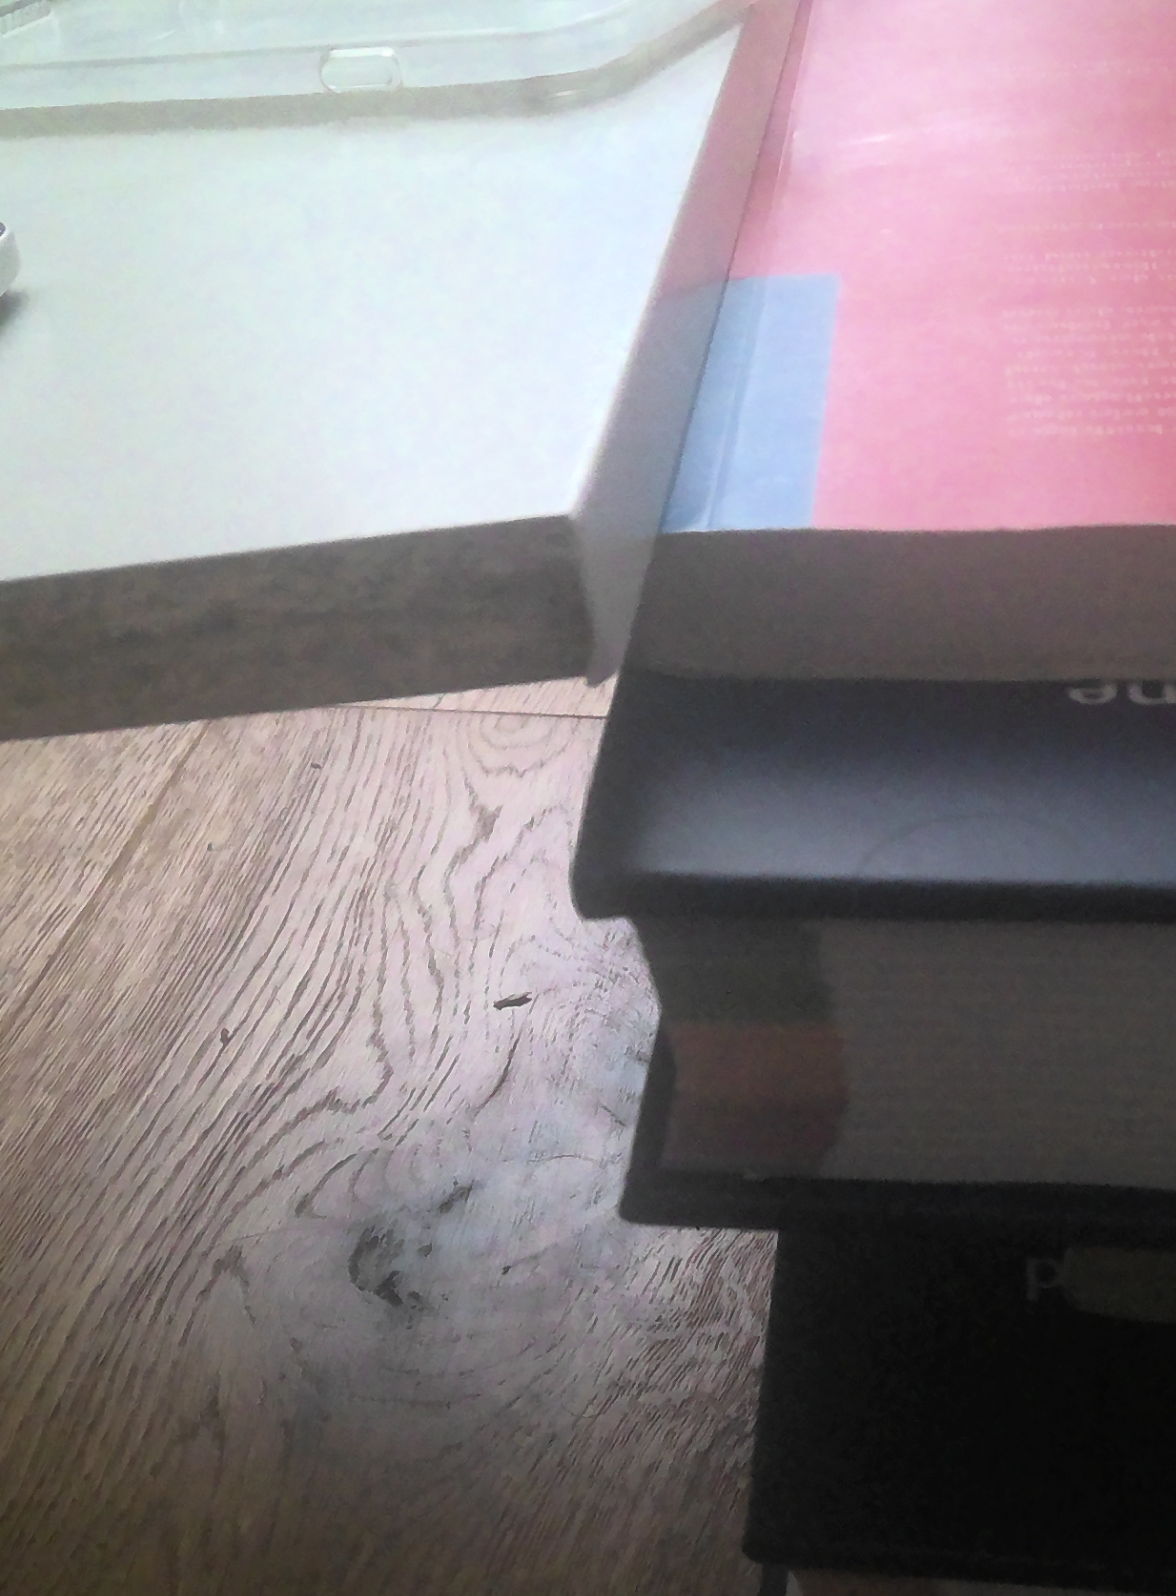
\includegraphics[width=\linewidth]{pics/buchstapel.png}
        \caption[Aufbau des Experiments Bücherstapel]{Aufbau des Bücherstapels}
        \label{fig:buchstapel}
        \end{minipage}
    \end{minipage}
 \end{figure}


\section{Geräteliste}
\label{sec:geraeteliste}
%\setlength\LTleft{-6.5em}
\begin{longtable}{c|c|S|p{15em}}
\caption[Geräteliste]{Verwendete Geräte \label{tab:geraeteliste}} \\  % optionales Argument wird in Verzeichnissen verwendet, essentielles Argument direkt im Text
\toprule
Gerät                              & Gerät-Nr. & { Unsicherheit }  & Bemerkungen \\  
\midrule
\endfirsthead
\caption[]{(Fortsetzung)}\\
\toprule
Gerät                              & Gerät-Nr. & { Unsicherheit }  & Bemerkungen \\                                                                        
\midrule
\endhead
\endfoot
\endlastfoot
Brett & axx & \SI{119.0(1)}{\cm}       & Ist die Roll bzw. Rutschebene für die Objekte\\ \hline
        Maßband         & bxx & \SI{1}{\mm}       & Um die Länge des Brettes und die Höhe der hohen Bücherstapel zu messen \\ \hline
        Schublehre      & cxx & \SI{0.02}{\mm}    & Um die Höhe der niedrigen Bücherstapel zu messen \\ \hline
        Bücher 13x & dxx & { - }             & Um die Höhe des Dreiecks der schiefen Ebene genau einstellen zu können\\ \hline
        Stuhl       & fxx & { - }             & Wurde verwendet als Gegenkathete für die Bestimmung des Gleitreibungskoeffizienten\\ \hline
        Smartphone     & hxx & { - }             & Um den Winkel mittels Phyphox zu messen und den Bewegungvorgang bei der Gleitreibung aufzuzeichnen\\ \hline
        Gummiball      & ixx & { - }             & Um den Rollreibungskoeffizienten von Gummi auf laminiertem Holz zu bestimmen \\ \hline
        PET-Handy Hülle     & jxx & {-} & Um Haft- und Gleitreibungskoeffizient von PET auf laminiertem Holz zu bestimmen\\ \hline
        \hline
\end{longtable}

\section{Versuchsdurchführung und Messergebnisse}
\label{sec:versuchsdurchfuehrung_messergebnisse}

\subsection{Reibung}
Wie in \nameref{sec:voraussetzungen_grundlagen} beschrieben, ist
es notwendig den genauen Winkel zu bestimmen, bei dem das Handy mit
der Gummihülle zu rutschen beginnt. Dieser Winkel 
wurde mit den Büchern genau bestimmt, da diese es einem erlauben
den Winkel präzise einzustellen. Hier wurde sowohl 
die App Phyphox, als auch gute alte Distanzmessung verwendet um den
Winkel zu bestimmen:

\begin{table}[H]
    \centering
    \caption{Werte damit der Haftreibungskoeffizient $\mu_H$ nach
        \autoref{eq:gleit} bestimmt werden 
    kann. \\
    $\alpha$ der Grenzwinkel der schiefen Ebene, bei dem sich das Objekt zum Bewegen beginnt\\
    $l$ ist die Hypothenuse, also die Länge des Bretts \\
    $h$ ist die Höhe des Bücherstapels \\
}
    \label{tab:messwerte_haft}
    \begin{tabular}{c|S|S}
        Symbol & {Wert} & {$\Delta$} \\ \hline
        $\alpha$ / \si{\degree} & 18.37 & +-0.10 \\
        $l$ / \si{\cm} & 118.8 & +-0.2 \\
        $h$ / \si{\cm} & 37.3 & +-0.2 \\
    \end{tabular}
\end{table}

Da die, anfangs noch doppelt gemessenen, Winkel genau übereinstimmen, wird bei
der Bestimmung des Gleitreibungskoeffizienten nur mehr die App für die
Winkelmessungen verwendet.

Bei der Gleitreibung, wie in \autoref{eq:gleit} ersichtlich, müssen der Winkel
$\alpha$ der schiefen Ebene und die Zeit $t$, welche das Objekt gebraucht hat um
die Distanz $s$ zurückzulegen, bestimmt werden. Die erhaltenen
Werte sind in folgender Tabelle ersichtlich:

\begin{table}[H]
    \centering
    \caption{Werte damit der Gleitreibungkoeffizient nach \autoref{eq:gleit} bestimmt werden 
    kann. \\
    $\alpha$ der Grenzwinkel der schiefen Ebene \\
    $s$ die zurückgelegte Distanz in einer Zeit $t$ \\
}
    \label{tab:messwerte_gleit}
    \begin{tabular}{c|S|S}
        Symbol & {Wert} & {$\Delta$} \\ \hline
        $\alpha$ / \si{\degree} & 24.03 & +-0.03\\
        $s$ / \si{\cm} & 57.0 & +-0.1 \\
    \end{tabular}
\end{table}

Die Zeit wurde bestimmt, indem der Rutschvorgang mittels Slow-Motion aufgezeichnet
wurde. Folgende Werte sind erhalten worden, mit der Annahme, dass die Zeitmessungen normalverteilt sind:

\begin{table}[H]
    \centering
    \caption{Dies sind die Zeitwerte damit mit \autoref{tab:messwerte_gleit} 
        der Gleitreibungkoeffizient nach \autoref{eq:gleit} bestimmt werden 
    kann. \\
    $t$ die Zeit, welche das Objekt gebraucht hat um die Distanz $s$ zurückzulegen \\
    Alle Werte sind mit $\Delta t$ = \SI{0.008}{\second} bestimmt worden
    und die Einheit aller Werte sind Sekunden.
}
    \label{tab:messwerte_gleit_zeit}
    \begin{tabular}{c|S|S}
        i & {$t$} \\ \hline
        1 & 0.883 \\
        2 & 0.858 \\
        3 & 0.870 \\
        4 & 0.916 \\
    \end{tabular}
\end{table}

\begin{figure}[H]
    \centering
    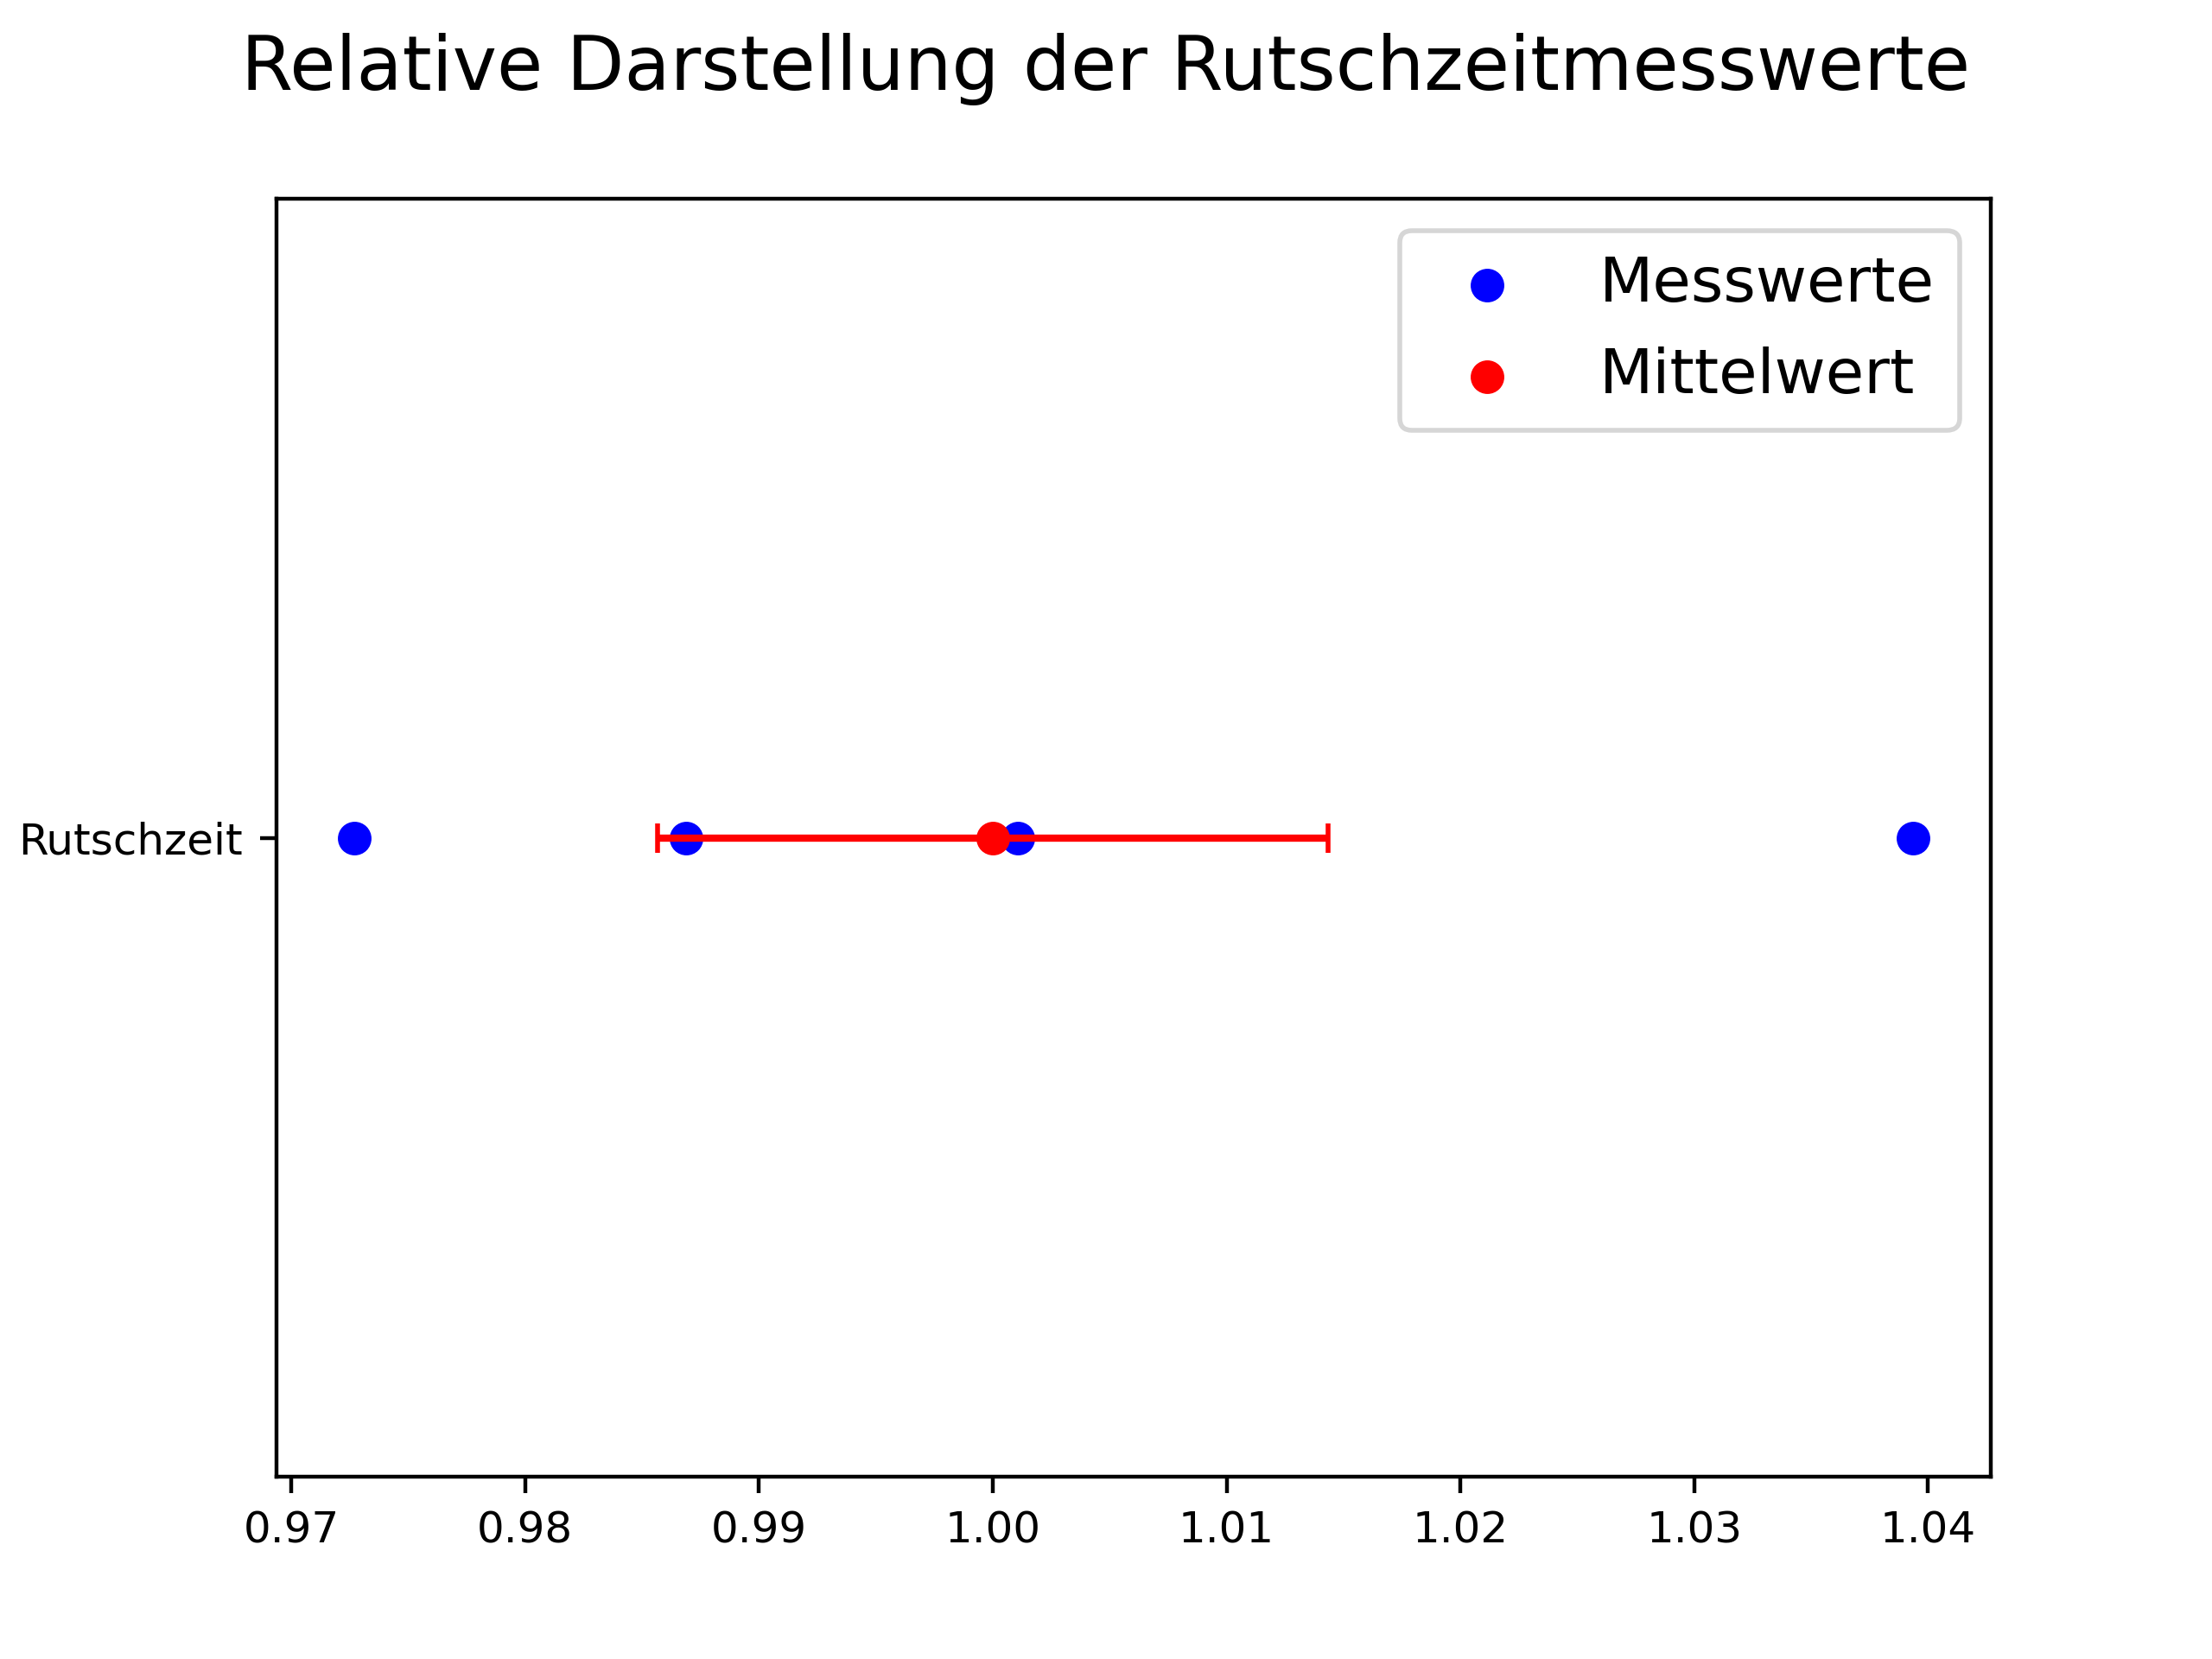
\includegraphics[width=0.8\linewidth]{pics/Rutschzeitmesswerte.png}
    \caption{Dieses Bild stellt die gemessen Zeiten relativ zum Mittelwert dar. Damit die Verteilung der
    Messwerte gut ersichtlich ist}%
    \label{fig:pics/Rutschzeitmesswerte}
\end{figure}

Bei der Rollreibung, ist man ähnlich vorgegangen, wie bei der Haftreibung.
Es muss, wie in \autoref{eq:roll} ersichtlich, auch ein Grenzwinkel
$\alpha$ bestimmt werden, jedoch ist dies der Winkel bei dem ein Zylinder
oder Kugel zu rollen beginnt. Hier ist der Winkel auch mittels
Pythagoras bestimmt worden. Zudem war es möglich die kleine
Buchstapelhöhe $h$ mit einer Schublehre zu bestimmen. Folgende Werte 
sind bei den Messungen erhalten worden:


\begin{table}[H]
    \centering
    \caption{Werte damit der Rollreibungskoeffizient $\mu_R$ nach
        \autoref{eq:roll} bestimmt werden 
    kann. \\
    $\alpha$ der Grenzwinkel der schiefen Ebene, bei dem sich das Objekt zu bewegen beginnt\\
    $l$ ist die Hypothenuse, also die Länge des Bretts \\
    $h$ ist die Höhe des Bücherstapels \\
    $d$ ist der Durchmesser des Gummiballs \\
}
    \label{tab:messwerte_roll}
    \begin{tabular}{c|S|S}
        Symbol & {Wert} & {$\Delta$} \\ \hline
        $l$ / \si{\cm} & 118.8 & +-0.2 \\
        $h$ / \si{\mm} & 20.96 & +-0.06\\
        $d$ / \si{\mm} & 37.78 & +-0.04\\
    \end{tabular}
\end{table}

\subsection{Viskosität}
Nun zu den Viskositätsversuch, da die benötigten Materialien nicht vorhanden waren, war es leider nicht möglich, dieses
Experiment, wie es in \nameref{sec:versuchsanordnung} beschrieben ist, durchzuführen.
Daher kann die genaue Vorgehensweise nicht beschreiben werden. 
Eine Möglichkeit hierzu, wäre die Dichte vom Medium und der Stahlkugel
aus einer Literaturquelle zu entnehmen und den Radius der Kugel mit einer Schublehre zu messen. 
Weiters muss wie in \autoref{eq:stokes} ersichtlich die 
finale Fallgeschwindigkeit der Kugel bestimmt werden, 
welche zB. durch das Aufzeichnen mit einer Kamera und 
einem Lineal auf der Seite gemacht werden kann, jedoch 
sollte die Brechung nicht vergessen werden. Spherische
Gefäße sollten aus Komplexität der Rechnung vermieden werden (Brechung an Kreisoberfläche).

Jedoch wurde in diesem Experiment angenommen, dass sich die Kugel 
schon lange genung in der Flüssigkeit befindet, sodass sie
ihre Terminalgeschwindigkeit schon erreicht hat und 
man bei einer Fallhöhe $h$ beginnt die Zeit $t$ zu messen,
die die Kugel benötigt um den Boden zu erreichen.


%Nun zu den Viskositätsversuch, da mir die Mittel fehlen, dieses
%Experiment wie es in \nameref{sec:versuchsanordnung} durch zu führen
%kann ich keine genau Vorgehensweiße beschreiben. Aber
%ein Möglichkeit wäre die Dichte vom Medium und der Stahlkugel
%aus einer Quelle nehmen und den Radius der Kugel zu messen. 
%Weiters muss wie in \autoref{eq:stokes} ersichtlich die 
%finale Fallgeschwindigkeit der Kugel bestimmt werden, 
%welche zb. durch das Aufzeichen mit einer Kamera und 
%einem Lineal auf der Seite gemacht werden kann, jedoch 
%sollte die Brechnung nicht vergessen werden. Spherische
%Gefäße sollten aus Komplexität der Rechnung vermieden werden (Brechung an Kreisoberfläche).
%
%Jedoch wurde in diesem Experiment angenommen, dass die Kugel sich
%schon in Flüssigkeit lange genung befindet, sodass sie
%ihre Terminalgeschwindigkeit schon erreicht hat und 
%man einer Fallhöhe $h$ beginnt die Zeit $t$ zu messen
%die die Kugel benötigt den Boden zu erreichen.

Hier wurden die vorgegebenen Werte verwendet.

\begin{table}[H]
    \centering
    \caption{Systemgrößen des Viskositätsversuch:\\
    $d$ Durchmesser der Stahlkugel\\
    $\rho_{Stahl}$ Dichte von Stahl\\
    $\rho_{Öl}$   Dichte von Speiseöl\\
    $h$           Fallhöhe\\
    $D$          Durchmesser des Gefäßes\\ 
    Werte wuder aus der Vorgabe \cite{werteviskositat} entnommen.
}
    \label{tab:system_viskosität}
    \begin{tabular}{c|S|S}
        Symbol                                & {Wert} & {$\Delta$} \\ \hline
        $d$            / \si{\mm}             & 1.05       & +-0.10 \\
        $\rho_{Stahl}$ / \si{\g\per\cm\cubed} & 7.85       & { - } \\
        $\rho_{Öl}$    / \si{\g\per\cm\cubed} & 0.92       & { - } \\
        $h$            / \si{\mm}             & 500    & +-2\\
        $D$            / \si{\mm}             & 80     & +-0.5\\
    \end{tabular}
\end{table}

Folgende Werte sind für die Fallzeit, die die Kugel
benötigt hat um zum Boden zu gelangen, bestimmt worden:


\begin{table}[H]
    \centering
    \caption{Die nötige Zeit $t$ die eine Stahlkugel (in Öl)
        braucht um von der Fallhöhe $h$ = \SI{500(2)}{\mm} zum
        Boden des Gefäßes zu gelangen. Die Zeitmessungen haben eine Unsicherheit
        von \SI{+-0.10}{\second}. Werte wurden aus der Vorgabe \cite{werteviskositat} entnommen.
}
    \label{tab:zeitmessungen_viskositat}
    \begin{tabular}{S}
        {$t$ / \si{\second}}  \\ \hline
         10.70                \\
         10.72                \\
         10.77                \\
         10.90                \\
         10.84                \\
    \end{tabular}
\end{table}

\begin{figure}[H]
    \centering
    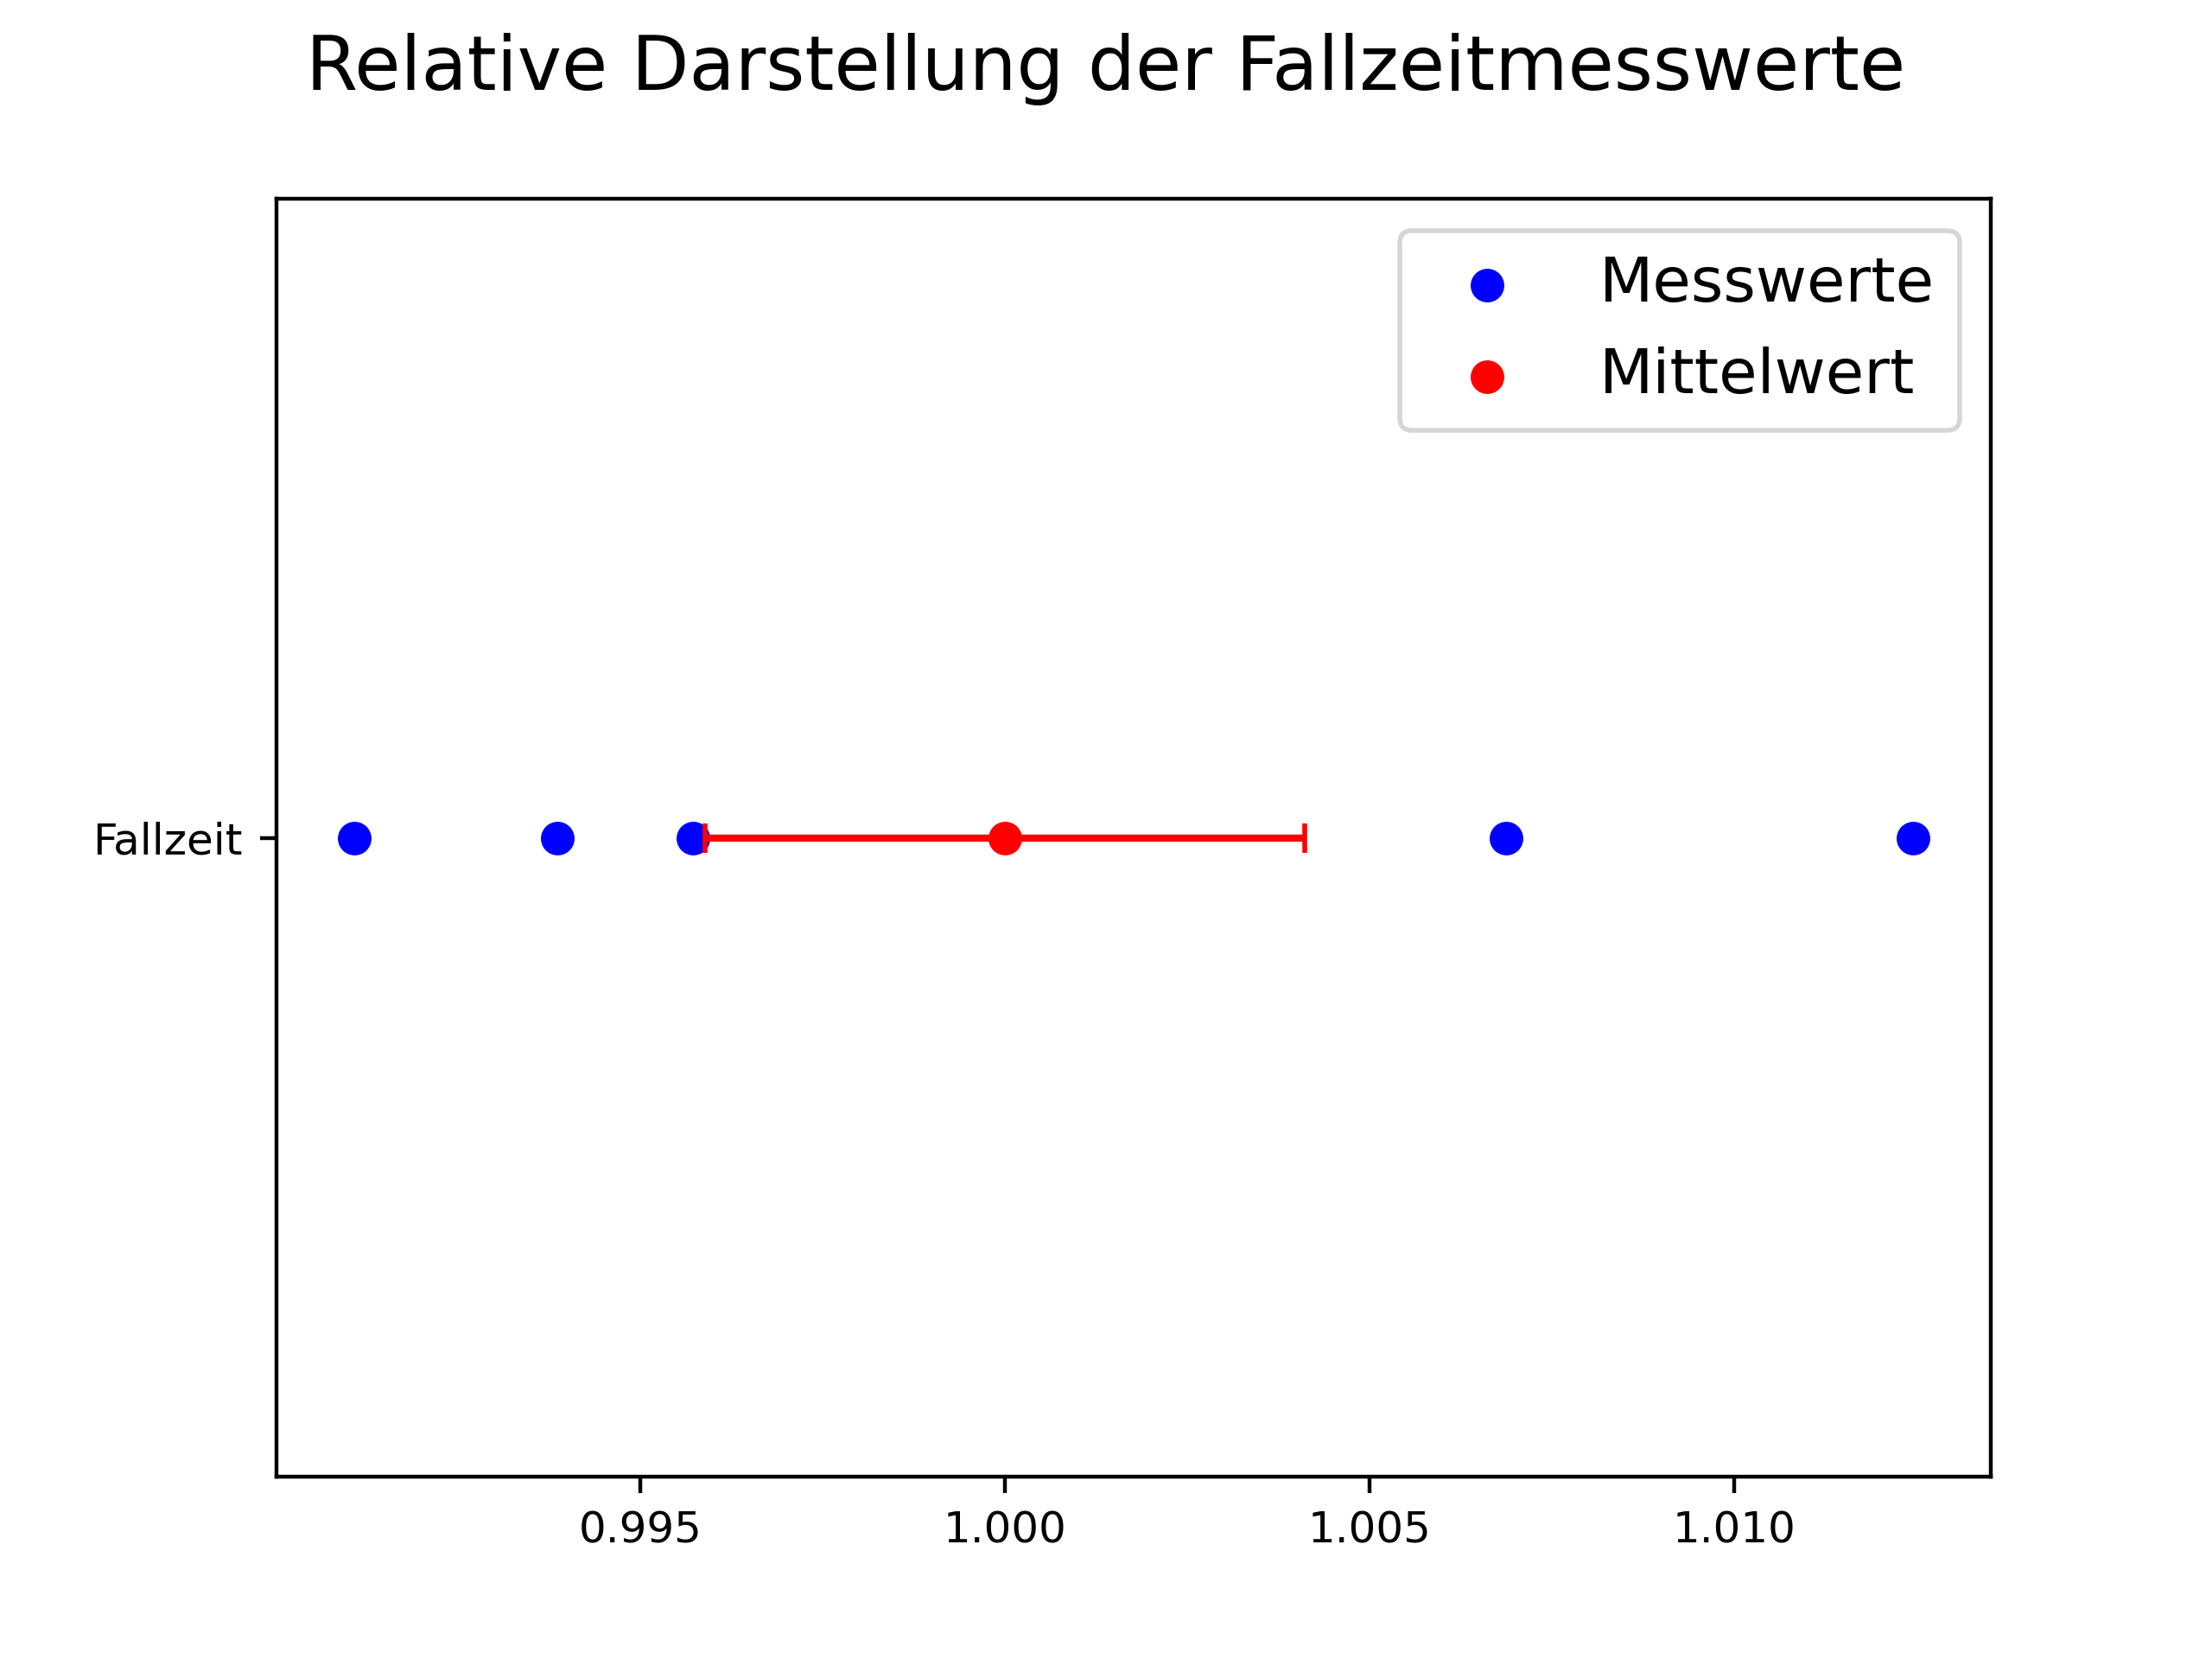
\includegraphics[width=0.8\linewidth]{pics/Fallzeitmesswerte.png}
    \caption{Dieses Bild stellt die gemessen Zeiten relativ zum Mittelwert dar. Damit die Verteilung der
    Messwerte gut ersichtlich ist}%
    \label{fig:pics/Fallzeit}
\end{figure}
\section{Auswertung}
\label{sec:auswertung}

\subsection{Reibung}
Nimmt man nun die Werte aus \autoref{tab:messwerte_haft} und
setzt diese in \autoref{eq:haft} ein, erhält man folgende Werte
für den Haftreibungskoeffizient $\mu_H$:

\begin{align}
    \mu_H &= \num{0.332(2)} \quad \text{mit der App} \\
    \mu_H &= \num{0.331(3)} \quad \text{mit Längenmessung}
\end{align}

Mittelt man nun die Werte, aus \autoref{tab:messwerte_gleit_zeit}
$\bar{t}=\SI{0.882(13)}{\second}$ und nimmt die restlichen Werte von
\autoref{tab:messwerte_gleit} und wendet diese Wert auf \autoref{eq:gleit} an,
bekommt man einen Wert für den Gleitreibungskoeffizient $\mu_G$:

\begin{equation}
    \mu_G = \num{0.282(5)}
\end{equation}

Als Nächstes wird der Rollreibungskoeffizient mit den Daten aus \autoref{tab:messwerte_roll}
und der \autoref{eq:roll} bestimmt und dadurch folgender Wert gefunden:

\begin{equation}
    \mu_R = \SI{0.0003333+-0.0000012}{\meter}
\end{equation}

\subsection{Viskosität}
Nun zu den Teil des Experiments, der sich mit der Viskosität von Öl
beschäftigt. 

Mittelt man die Zeiten, aus den durchgeführten Messungen, erhält
man den durchschnittlichen Wert für die Fallzeit: 

\begin{equation}
    \bar{t} = \SI{10.77(10)}{\second}
\end{equation}

Unter Annahme, dass die Kugel ihre Terminalgeschwindigkeit $v$ schon
erreicht hat, wenn die Messung beginnt, ergibt sich für $v=\frac{h}{t}$. Wobei
$h$ die Fallhöhe und $t$ die zuvor errechnete Fallzeit ist. Durch
Einsetzen erhält man:
\begin{equation}
    v = \SI{4.64(5)}{\cm\per\second}
\end{equation}

Mit dem Wert von $v$ und den anderen Werten aus \autoref{tab:system_viskosität}
kann mit \autoref{eq:viskositat} die Viskosität von Öl bestimmmt werden:

\begin{equation}
    \eta = \SI{90(17)}{\milli\Pa\second}
\end{equation}

Mit diesen Werten lässt sich die Reynoldzahl Re des
Systems finden:

\begin{equation}
    \text{Re} = \num{0.50(5)}
\end{equation}


\section{Diskussion und Zusammenfassung}
\label{sec:diskussion_zusammenfassung}
% Aufzählung was scheiße glaufen is

Nun werden die verwendeten Methoden diskutiert und die Ergebnisse 
zusammengefasst.

\subsection{Reibung}
Durch Aufzeichen der dynamischen Messungen und der genauen Höheneinstellung
mittels Bücher war es möglich, sehr genaue Werte für den Reibungsteil des
Experiments zu bestimmen. Weiters war die Phyphox App überraschenderweise sehr
genau.

Die, hier verwendete, Definition der Rollreibung \ref{eq:roll} wird in der
Literatur nicht wirklich verwendet, deshalb werden beim Vergleich der Literatur
mit dem Radius $r$ der Kugel multipliziert. Zudem war es nur möglich den
Rollreibungskoeffizienten von Autoreifen auf Beton
\cite{Rollwiderstandgummi2021} zu finden, deshalb ist wie erwartet der gemessen
Rollreibungskoeffizient im unterem Ende des Spektrums von Beton. Da laminiertes
Holz rutschiger ist.

Auch ist noch anzumerken, dass die getätigte Annahme, dass die Kugel in der
viskosen Flüssigkeit bereits die Terminalgeschwindigkeit erreicht hat,
möglicherweise falsch ist. Wenn das der Fall wäre, würde man eine Aufzeichnung
des Bewegungvorgangs (Ort und Zeit) brauchen. Da es nicht möglich wäre ohne das
Wissen über die Viskosität der Flüssigkeit die Bewegunggleichung zu lösen.

Alle erhaltenen Werte beinhalten die
Literaturwerte in ihren Unsicherheitsintervallen, siehe
\autoref{tab:ergebnisse}.

\begin{table}[H]
    \centering
    \caption{Hier werden die erhaltenen Werte den Literaturwerten gegenübergestellt.\\
    $\mu_H$ der Haftreibungskoeffizient von einer PET Handyhülle auf einem laminierten Holzbrett\\ 
    $\mu_G$ der Gleitreibungkoeffizient von einer PET Handyhülle auf einem laminierten Holzbrett\\
    $\mu_R$ der Rollreibungskoeffizient von einem Gummiball auf einem laminierten Holzbrett\\
    $\eta$ die Viskosität von Öl\\
    }
    \label{tab:ergebnisse}
    \begin{tabular}{c|S[table-format=2.7(7)]|S}
        Symbol:                   & {Bestimmter Wert}                  & {Literaturwert}           \\ \hline
        $\mu_H$ /                 & 0.332(2) & 0.33  \cite{Kurdi2018}    \\
        $\mu_G$ /                 & 0.282(5) & \numrange{0.2}{0.5}	\cite{gleitreibung_pet} \cite{Filippova2016}  \\
        $\mu_R$ / \si{\meter}     & 0.0003333+-0.0000012 & {\numrange{0.0002}{0.0007} auf Beton} \cite{Rollwiderstandgummi2021}     \\
        $\eta$ / \si{\milli\Pa\second} & 90(17) & 100 \cite{viskositatöl2021}   \\
    \end{tabular}
\end{table}

Wie in \autoref{fig:pics/ergebnisse} ersichtlich sind die haben die erhaltenen Reibungskoeffizienten eine
niedrige relative Unsicherheit und entsprechen, wie in \autoref{tab:ergebnisse} ersichtlich, auch
den Literaturwert. Somit unterstützt dieses Experiment die in der Literatur gefunden Werte.


\begin{figure}[H]
    \centering
    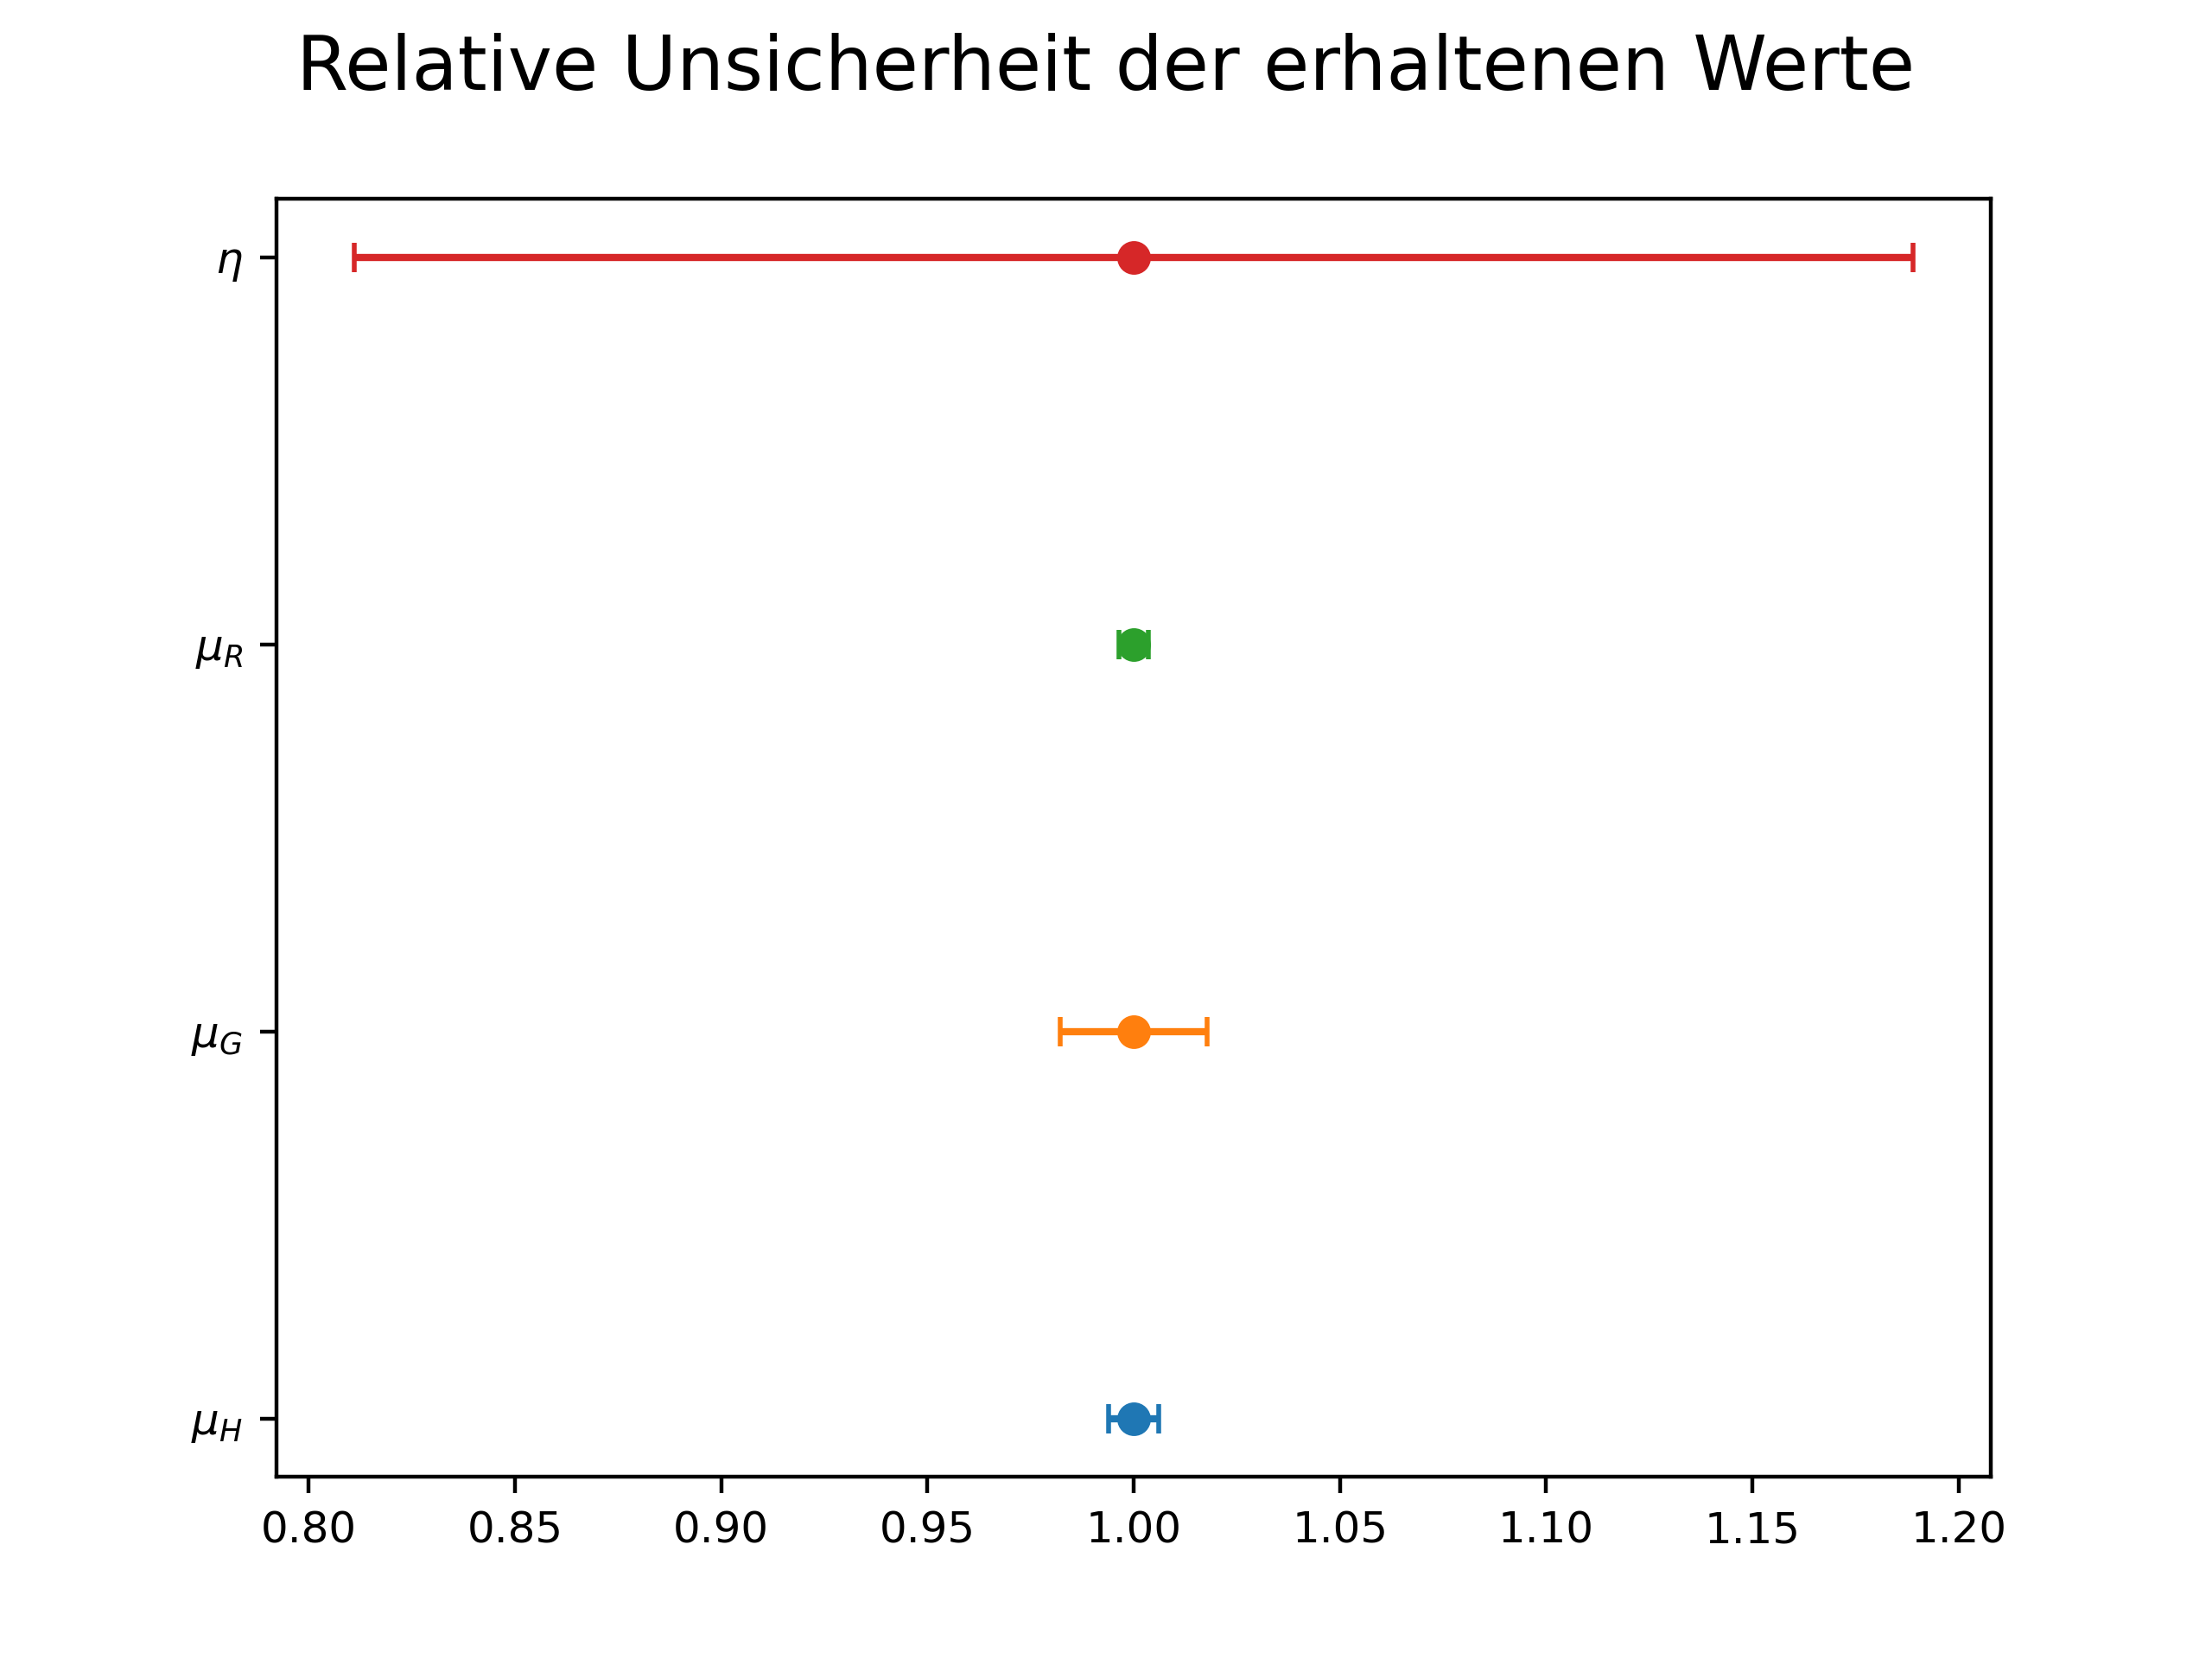
\includegraphics[width=0.8\linewidth]{pics/ergebnisse.png}
    \caption{Dieses Diagramm soll die Relative Unsicherheit der gemessen Werte visualisieren.\\
    $\mu_H$ der Haftreibungskoeffizient von einer PET Handyhülle auf einem laminierten Holzbrett\\ 
    $\mu_G$ der Gleitreibungkoeffizient von einer PET Handyhülle auf einem laminierten Holzbrett\\
    $\mu_R$ der Rollreibungskoeffizient von einem Gummiball auf einem laminierten Holzbrett\\
    $\eta$ die Viskosität von Öl\\
    }%
    \label{fig:pics/ergebnisse}
\end{figure}


Die zu messenden Winkel und Distanzen konnten sehr genau bestimmt werden, würde
man noch genauer messen wollen müsste man Effekte von Temperatur berücksichtigt
werden. Daher wäre es zu Empfehlen, wenn genauere Werte für die
Reibungskoeffizienten notwendig wären, auf ein Modell zu wechseln. Für die
Rollreibung zum Beispiel ein Modell mit Schwingungen in einem Topf um zu
steigen.  Wo die Schwingungsdauer und die Amplitude der Schwingung zu bestimmen
wären um einen Ausdruck für den Rollreibungskoeffizient in Abhängikeit der
Amplituden zu bekommen.

Um genauer Werte für die Viskosität zu bestimmen sollte, muss die Fallzeit
und besonders der Radius der Kugel genauer bestimmt werden.

Schlussendlich lässt sich sagen, dass die Methoden zureichend waren
um die gesuchten Werte zu bestimmen.
% Literaturtabelle
\newpage
\printbibliography

\listoffigures

\listoftables


\end{document}
